\chapter{Graphes}

\section{Définition}

\begin{definition}[Graphe]\index{Graphe}
Un graphe est constitué d'un ensemble de sommets $S$ d'un ensemble d'arêtes $A \subseteq S \times S$ reliant les sommets. Les arêtes sont orientées (flèche) ou non orientées (segment).
\end{definition}

\begin{notation}
On note un graphe $G = (S,\, A)$ en français, $G = (V,\, E)$ en anglais.
\end{notation}

\begin{figure}[h]
\centering
\begin{minipage}{.5\textwidth}
  \centering
  	\begin{tikzpicture}
		\GraphInit[vstyle=Hasse]
		\tikzset{VertexStyle/.append  style={fill = node}}
		\SetGraphUnit{3}
		\Vertex{A}
		\EA(A){B}
		\Edge(A)(B)
	\end{tikzpicture}
  \caption{Graphe non orienté}
  %\label{fig:test1}
\end{minipage}%
\begin{minipage}{.5\textwidth}
  \centering
  	\begin{tikzpicture}
		\GraphInit[vstyle=Hasse]
		\tikzset{VertexStyle/.append  style={fill = node}}
		\SetGraphUnit{3}
		\Vertex{A}
		\EA(A){B}
		\Edge[style={->}](A)(B)
	\end{tikzpicture}
  \caption{Graphe orienté}
\end{minipage}%
\end{figure}

Les sommets peuvent représenter des villes, des stations de métro, des sites sur des cartes géographiques, etc. Les arêtes peuvent symboliser des routes, des câbles, des liens, etc. Un graphe peut ainsi représenter des cartes géographiques, le web, les réseaux sociaux, des modèles 3D (animations), modèles physiques d'interactions...
%Comme on le voit sur la fig.~\ref{fig:test2}

\section{Représentations}

\begin{figure}[h]
	\centering
	\begin{tikzpicture}
		\GraphInit[vstyle=Normal]
		\tikzset{VertexStyle/.append  style={fill = node}}
		\tikzset{VertexStyle/.append  style={text = white}}
		\SetGraphUnit{1.5}
		\begin{scope}[rotate=90]
		\Vertices{circle}{1, 2, 4, 3}
		\Edge(1)(2)
		\Edge(1)(3)
		\Edge(3)(2)
		\Edge(4)(2)
		\Edge(4)(3)
		\SOEA(3){5}
		\WE(5){6}
		\Edge(5)(6)
		\end{scope}
	\end{tikzpicture}
	\caption{Graphe non orienté}
	\label{fig:chap1_graph1}
\end{figure}

\begin{figure}[h]
	\begin{minipage}{.5\textwidth}
		\begin{center}
		\begin{tabular}{| c | c | c | c | c | c | c |}
		\hline
		  & 1 & 2 & 3 & 4 & 5 & 6 \\ \hline
		1 & 0 & 1 & 1 & 0 & 0 & 0 \\ \hline
		2 & 1 & 0 & 1 & 1 & 0 & 0 \\ \hline
		3 & 1 & 1 & 0 & 1 & 0 & 0 \\ \hline
		4 & 0 & 1 & 1 & 0 & 0 & 0 \\ \hline
		5 & 0 & 0 & 0 & 0 & 0 & 1 \\ \hline
		6 & 0 & 0 & 0 & 0 & 1 & 0 \\
		\hline
		\end{tabular}
		\end{center}
		\caption{Matrice d'adjacence du graphe \ref{fig:chap1_graph1}}
	\end{minipage}
	\begin{minipage}{.5\textwidth}
		\begin{center}
		\begin{tabular}{| c | c  c  c | }
		\hline
		1 & 2 & 3 & \\ \hline
		2 & 1 & 3 & 4 \\ \hline
		3 & 1 & 2 & 4 \\ \hline
		4 & 2 & 3 & \\ \hline
		5 & 6 & & \\ \hline
		6 & 5 & & \\
		\hline
		\end{tabular}
		\end{center}
		\caption{Liste d'adjacence du graphe \ref{fig:chap1_graph1}}
	\end{minipage}
\end{figure}

\subsection{Matrice d'adjacence}\index{Matrice d'adjacence}
Une matrice d'adjacence pour un graphe $G$ à $n$ sommets est une matrice de dimension $n \,\times\, n$ dont où l'élément à la position $i,\,j$ vaut $1$ s'il existe une arête reliant le sommet $i$ au sommet $j$, $0$ sinon.

\subsection{Liste d'adjacence}\index{Liste d'adjacence}
Une liste d'adjacence est la liste des voisins de chaque sommets. C'est une représentation relativement compacte lorsqu'il y a peu d'arêtes.

\section{Chemins}
\begin{definition}[Chemin]\index{Chemin}
Un chemin de longueur $k$ de $u$ à $v$ dans un graphe $G = (S,\, A)$ est une suite de sommets $u_{0},\, u_{1},\, ...\, u_{k}$ telle que $u_{0} = u$, $u_{k} = v$ et on ne passe que par des arêtes de $G$. $\forall i \in \llbracket 0,\, k \rrbracket \in A$
\end{definition}

\begin{definition}[Chemin simple]\index{Chemin simple}
Un chemin simple est un chemin qui ne passe pas 2 fois par le même sommet.
\end{definition}

Exemples sur la figure \ref{fig:chap1_graph1} :
\begin{itemize}
\item 1, 3, 2, 4 est une chemin de longueur 3, de 1 à 4.
\item 1, 4, 5 n'est pas un chemin.
\end{itemize}

\section{Cycle}
\begin{definition}[Cycles]\index{Cycle}
Pour $u \in S$, un cycle est un chemin de longueur supérieure ou égale à 3, de $u$ à $u$, qui ne passe pas deux fois par le même sommet. Le graphe de la figure \ref{fig:chap1_graph1} possède des cycles.
\end{definition}

\section{Connexe}
\begin{definition}[Connexe]\index{Connexe}
Un graphe est connexe si $\forall u, v \in S$ il existe un chemin de $u$ à $v$ dans $G$. Le graphe de la figure \ref{fig:chap1_graph1} n'est pas connexe. Le graphe de la figure \ref{fig:chap1_arbr1} est connexe.
\end{definition}

\section{Arbres}
\begin{definition}[Arbre]\index{Arbre}
Un arbre est un graphe connexe sans cycle.
\end{definition}

\begin{figure}[h]
	\centering
	\begin{tikzpicture}
		\GraphInit[vstyle=Hasse]
		\tikzset{VertexStyle/.append  style={fill = node}}
		\tikzset{VertexStyle/.append  style={text = white}}
		\SetGraphUnit{1}
		\Vertex{a}
		\NOWE(a){b}		\Edge(a)(b)
		\SetGraphUnit{1.414}
		\WE(b){c}		\Edge(c)(b)
		\SetGraphUnit{1}
		\NOEA(a){d}		\Edge(a)(d)
		\NOEA(d){e}		\Edge(d)(e)
		\SetGraphUnit{1.414}
		\EA(e){f}		\Edge(e)(f)
		\SetGraphUnit{1}
		\SOEA(e){g}		\Edge(e)(g)
		\SOWE(a){h}		\Edge(a)(h)
		\SetGraphUnit{1.414}
		\WE(h){i}		\Edge(h)(i)
		\SetGraphUnit{1}
		\SOEA(a){j}		\Edge(a)(j)
		\NOEA(j){k}		\Edge(j)(k)
		
	\end{tikzpicture}
	\caption{Arbre}
	\label{fig:chap1_arbr1}
\end{figure}

\section{Arbre couvrants}\index{Arbre couvrant}

\begin{definition}[Arbre couvrant]\index{Arbre couvrant}
Un arbre $T = (S,\, A^{\prime})$ couvre un graphe $G = (S,\, A)$ si $A^{\prime} \subseteq A$.
\end{definition}

Un graphe à $n$ sommets peut admettre jusqu'à $n^{n-1}$ arbres couvrants.

\section{Graphes valués}

\begin{definition}[Graphe valué]\index{Graphe valué}\index{Graphe pondéré}
Un graphe est valué (ou pondéré) lorsqu'on y associe une fonction de coût sur les arêtes : $w : S \times S \rightarrow \mathbb{R}^{+}$
\end{definition}

\begin{figure}[h]
	\centering
	\begin{tikzpicture}
		\GraphInit[vstyle=Hasse]
		\tikzset{VertexStyle/.append  style={fill = node}}
		\tikzset{VertexStyle/.append  style={text = white}}
		\SetGraphUnit{1.5}
		\begin{scope}[rotate=90]
		\Vertices{circle}{1, 2, 4, 3}
		\Edge[label=$1$](1)(2)
		\Edge[label=$4$](1)(3)
		\Edge[label=$2$](3)(2)
		\Edge[label=$4$](4)(2)
		\Edge[label=$1$](4)(3)
		\end{scope}
	\end{tikzpicture}
	\caption{Graphe non orienté}
	\label{fig:graph1value}
\end{figure}

\section{Algorithme de Kruskal (1956)}

L'algorithme de Kruskal (1956) permet de trouver un arbre couvrant minimal dans un graphe valué $G = (S,\, A)$ , $w : S \times S \rightarrow \mathbb{R}^{+}$.

\begin{enumerate}
	\item Trier les arêtes par ordre de coût.
	\item Parcourir toutes les arêtes $(u,\, v)$ dans cet ordre. Si $(u,\, v)$ ne forme pas de cycle, l'ajouter à l'arbre.
\end{enumerate}


\section*{À ne pas confondre}

Un \textbf{problème}\index{Problème} décrit sur chaque donnée quel est le résultat attendu. ex : tri, recherche.

La \textbf{structure de données}\index{Structure de données} décrit comment les données sont organisées et comment on y accède.

Un \textbf{algorithme} décrit le déroulement des étapes permettant de résoudre un problème.

Un \textbf{programme} (ou \textbf{implémentation}) est un choix des structures de données, des librairies, du langage, de l'interface...


\section*{Exercices}

\subsection*{Exercice 1 : Ordres de grandeur}

Donner les relations $(o, O, \theta)$ entre les fonctions $f$ et $g$ suivantes :

\begin{enumerate}

\item $f(n) = 2n$ et $g(n) = 5n+1$;
\item $f(n) = n^{2}$ et $g(n) = n^{3}$;
\item $f(n) = n^{2}$ et $g(n) = 2n^{2}+3n+5$;
\item $f(n) = 8(\log n)^{2} $ et $g(n) = n - 2$;
\item $f(n) = \log (n^{2})$ et $g(n) = \log n$;
\item $f(n) = 2^{n}$ et $g(n) = n^{10}$;
\item $f(n) = 2^{n+1}$ et $g(n) = 2^{n}$;
\item $f(n) = 2^{2n}$ et $g(n) = 2^{n}$.

\end{enumerate}

\subsection*{Exercice 2 : Représentation des arbres}
%\begin{exercise}
Un arbre (pas forcément binaire) peut être représenté de deux façons :
\begin{itemize}[leftmargin=2cm]
\item par les prédécesseurs : chaque nœud contient un pointeur vers son père.
\item par liste d'adjacence : chaque nœud contient la liste de tous ses fils.
\end{itemize}

\begin{enumerate}
\item Dessiner un arbre à 8 sommets et donner les deux façons de le représenter.
\item Proposer un algorithme qui transforme un arbre donné par liste d'adjacence en un arbre donné par prédécesseurs.
Évaluer sa complexité.
\item Donner un algorithme qui transforme un arbre donné par prédécesseurs en un arbre donné par liste d'adjacence.
Évaluer sa complexité.
\end{enumerate}

\vspace{0.2cm}

Solution : \url{https://cloud.sagemath.com/projects/bb22f23b-6876-4930-9368-3ea2c32cf718/files/Tree.sagews}
%\end{exercise}
